\section{Large-scale catchment water and salt balance model element (model ID: 23)}
The large-scale catchment water and salt balance model (LASCAM) (fig.~\ref{fig:23_schematic}) is part of a study that investigates soil water and salt concentration before and after forest clearing \citep{Sivapalan1996a}. It is a semi-distributed model made up of individual elements, such as described below. The model presented here simulates the water balance only (salt is ignored). It has 3 stores and 24 parameters ($\alpha_f$, $\beta_f$, $B_{max}$,  $F_{max}$, $\alpha_c$, $\beta_c$, $A_{min}$, $A_{max}$, $\alpha_{ss}$, $\beta_{ss}$, $c$, $\alpha_g$, $\beta_g$, $\gamma_f$, $\delta_f$, $t_d$, $\alpha_b$, $\beta_b$, $\gamma_a$, $\delta_a$, $\alpha_a$, $\beta_a$, $\gamma_b$ and $\delta_b$). The model aims to represent:

\begin{itemizecompact}
\item Stylized interception;
\item Saturation and infiltration excess surface runoff;
\item An inner layout representing near-stream saturated storage, deep saturated storage and medium-depth unsaturated storage;
\item Subsurface saturation and infiltration excess flow to the near-stream store;
\item Percolation to and capillary rise from groundwater.
\end{itemizecompact}

\subsection{MARRMoT model name}
m\_23\_lascam\_24p\_3s \\

% Equations
\subsection{Model equations}

% Model layout figure
{ 																	% This ensures it doesn't warp text further down
\begin{wrapfigure}{l}{5cm}
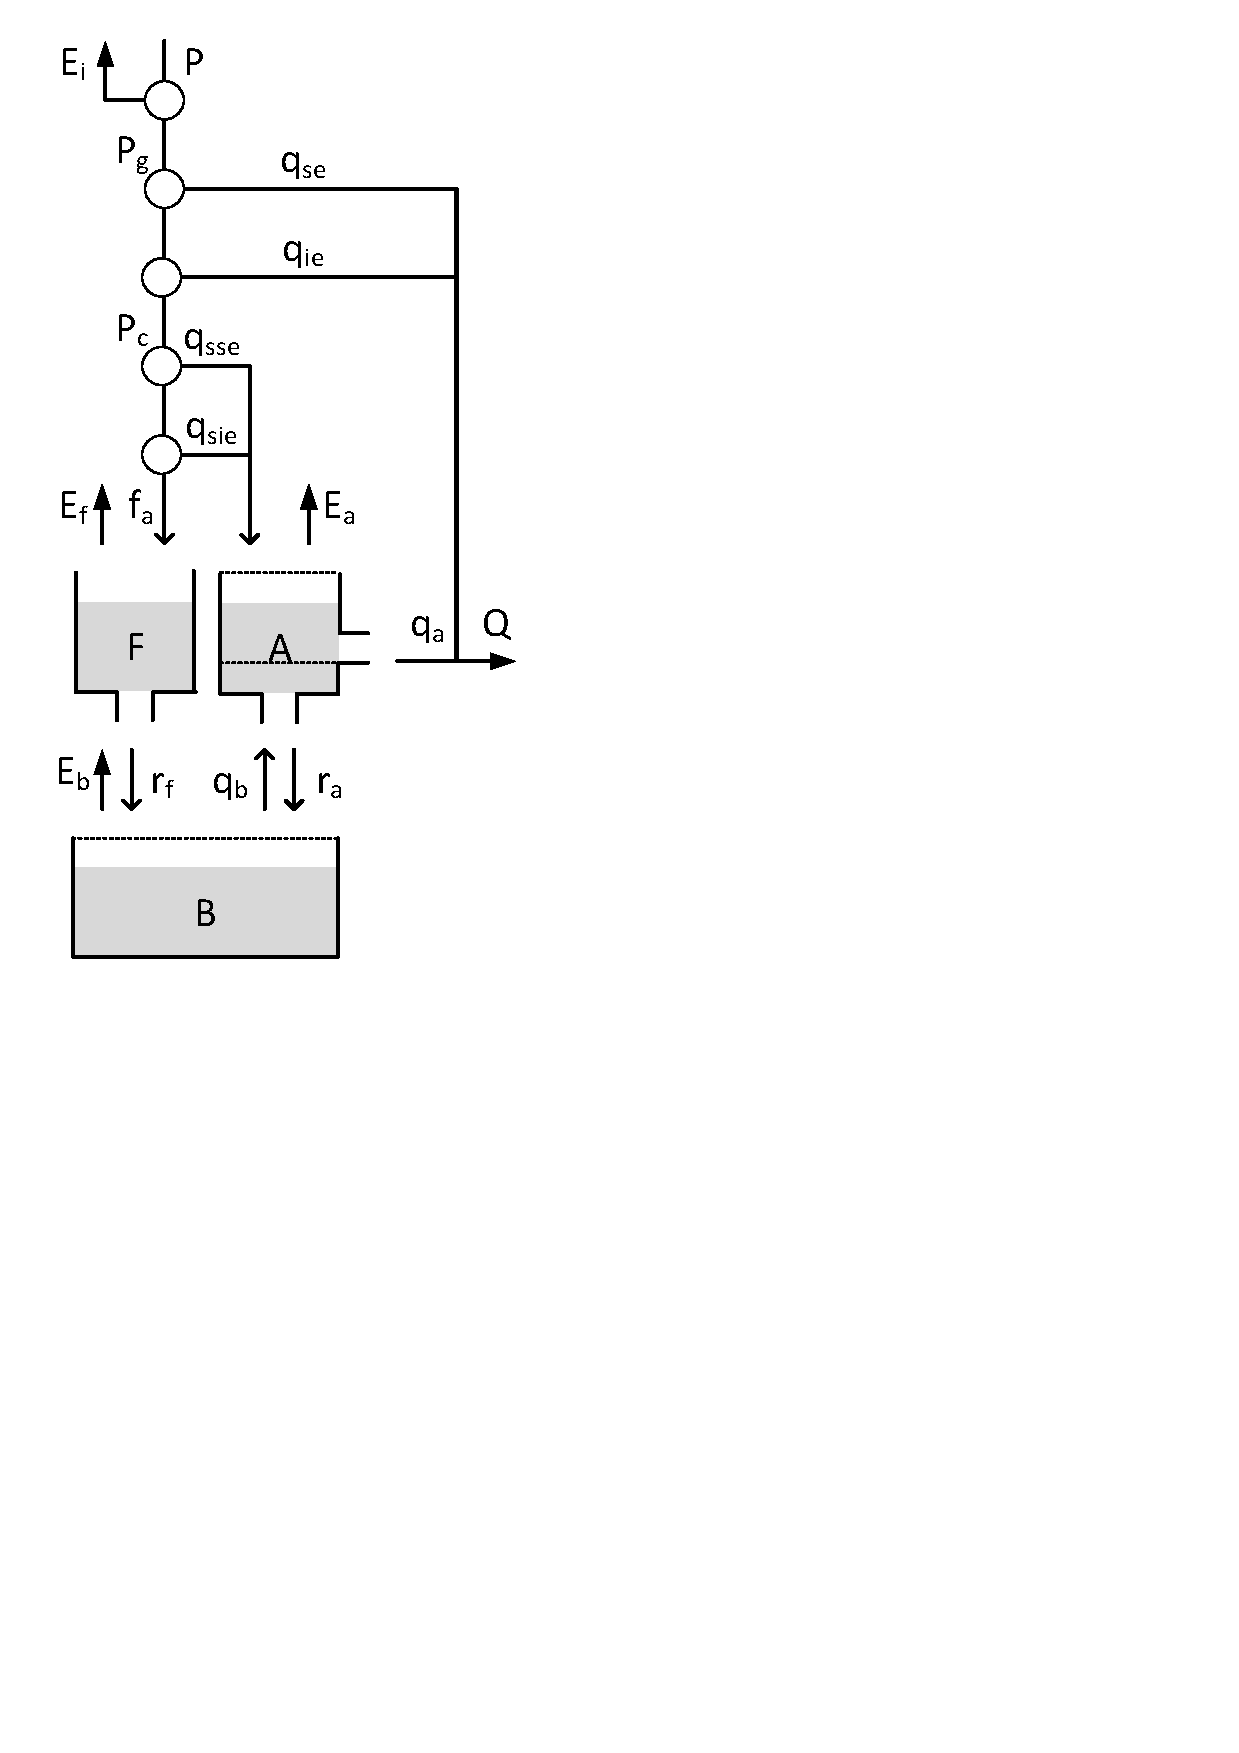
\includegraphics[trim=1cm 13.5cm 7cm 1cm,width=7cm,keepaspectratio]{./AppA_files/23_schematic.pdf}
\caption{Structure of the LASCAM model} \label{fig:23_schematic}
\end{wrapfigure}

\begin{align}
	\frac{dF}{dt} &= f_a-E_f-r_f \\
	f_a &= min\left(P_c*max\left(1,\frac{1-\phi_{ss}}{1-\phi_c}\right),f_{ss}^*\right) \\
	f_{ss}^* &= \alpha_f\left(1-\frac{B}{B_{max}}\right)\left(\frac{F}{F_{max}}\right)^{-\beta_f}\\
	\phi_c &= \begin{cases}
		\alpha_c\left(\frac{A-A_{min}}{A_{max}-A_{min}}\right)^{\beta_c}, &\text{if } A > A_{min} \\
		0, & \text{otherwise} \\
	\end{cases}\\
	\phi_{ss} &= \begin{cases}
		\alpha_{ss}\left(\frac{A-A_{min}}{A_{max}-A_{min}}\right)^{\beta_{ss}}, &\text{if } A > A_{min} \\
		0, & \text{otherwise} \\
	\end{cases}\\
	P_c &= min\left(P_g-q_{se},f^*_s\right) \\
	f^*_s &= c \\
	q_{se} &= \phi_c*P_g \\
	P_g &= max\left(\alpha_g+\beta_g*P,0\right)\\
	E_f &= \gamma_f*E_p\left(\frac{F}{F_{max}}\right)^{\delta_f}\\
	r_f &= t_d*F
\end{align}

} % end of wrapfigure fix

Where $F$ [mm] is the current storage in the unsaturated infiltration store, which controls the amount of subsurface runoff generated on the boundary of a more permeable top layer (store $A$) with a less permeable bottom layer (store $F$).
$F$ is refilled by actual infiltration $f_a$ $[mm/d]$, and drained by recharge $r_f$ $[mm/d]$ and evaporation $E_b$ $[mm/d]$. 
$f_a$ depends on the actual infiltration rate $P_c$ $[mm/d]$, the fraction saturated catchment area $\phi_{ss}$ [-], the fraction variable area contributing to overland flow $\phi_c$ [-] and a catchment-scale infiltration capacity $f_{ss}^*$ $[mm/d]$. 
$f_{ss}^*$ depends on a scaling parameter $\alpha_f$ $[mm/d]$, the relative storage in groundwater $B/B_{max}$, the relative infiltration volume in the catchment $F/F_{max}$ and non-linearity parameter $\beta_f$ [-]. 
$B_{max}$ [mm] and $F_{max}$ [mm] are storage scaling parameters [-].
$\phi_c$ uses the minimum contributing storage $A_{min}$ [mm], maximum contributing storage $A_{max}$ [mm] and shape parameters $\alpha_c$ [-] and $\beta_c$ [-] to control the shape of this distribution.
$\phi_{ss}$ takes a similar shape as $\phi_c$, using parameters $\alpha_{ss}$ [-] and $\beta_{ss}$ [-].
$P_c$ is the lesser of throughfall rate $P_g$  $[mm/d]$ minus saturation excess $q_{se}$  $[mm/d]$, and the catchment infiltration capacity $f_s^*$  $[mm/d]$.
$f_s^*$ is assumed to have a constant rate $c$  $[mm/d]$.
$q_{se}$ is determined as that part of throughfall $P_g$ that falls on the variable contributing catchment area given by $\phi_c$.
$P_g$ is determined as a fixed interception rate $\alpha_g$  $[mm/d]$ and a fractional interception $\beta_g$ [-].
Evaporation $E_f$ uses the potential rate $E_p$ $[mm/d]$  scaled by the relative storage in $F$ and two shape parameters  $\gamma_f$ [-]  and $\delta_f$ [-].
Recharge $r_f$ $[mm/d]$ has a linear relation with storage through time parameter $t_d$ $[d^{-1}]$.

\begin{align}
	\frac{dA}{dt} &= q_{sse} +q_{sie} + q_b - E_a - q_a - r_a\\
	q_{sse} &= \frac{\phi_{ss}-\phi_c}{1-\phi_c}P_c\\
	q_{sie} &= max\left(P_c*\frac{1-\phi_{ss}}{1-\phi_c}-f^*_{ss},0\right) \\
	q_b &= \beta_b\left(exp\left(\alpha_b\frac{B}{B_{max}}\right)-1\right) \\
	E_a &= \phi_c*E_p + \gamma_a*E_p\left(\frac{A}{A_{max}}\right)^{\delta_a}\\
	q_a &= \begin{cases}
		\alpha_a\left(\frac{A-A_{min}}{A_{max}-A_{min}}\right)^{\beta_a}, &\text{if } A > A_{min} \\
		0, & \text{otherwise} \\
	\end{cases}\\
	r_a &= \phi_{ss}*f^*_{ss}
\end{align}

Where $A$ [mm] is the current storage in the more permeable upper zone (above less permeable lower zone $F$), refilled by sub-surface saturation excess $q_{sse}$ $[mm/d]$, sub-surface infiltration excess $q_{sie}$ $[mm/d]$ and discharge from groundwater $q_b$ $[mm/d]$. 
The store is drained by evaporation $E_a$, subsurface stormflow $q_a$ $[mm/d]$ and recharge $r_a$ $[mm/d]$.
Flow from store $B$, $q_b$, decreases exponentially as the store dries out, controlled by parameters $\beta_b$ $[mm/d]$ and $\alpha_b$ [-]. 
Evaporation $E_a$ occurs at the potential rate $E_p$ from the variable saturated area $\phi_c$ and additionally at a rate scaled by the relative storage in $A$ and two shape parameters $\gamma_a$ [-] and $\delta_a$ [-].
Subsurface flow $q_a$ occurs only if current storage exceeds threshold $A_{min}$ and maximum rate $\alpha_a$ [mm/d], controlled by scaling parameter $\beta_a$ [-].
Recharge $r_a$ is a function of the saturated subsurface area $\phi_{ss}$ and the subsurface infiltration rate $f_{ss}^*$.

\begin{align}
	\frac{dB}{dt} &= r_f+r_a - E_b - q_b \\
	E_b &= \gamma_b*E_p\left(\frac{B}{B_{max}}\right)^{\delta_b}
\end{align}
  
Where $B$ [mm] is the current storage in the deep layers, refilled by recharge from stores A ($r_a$) and F ($r_f$), and drained by evaporation $E_b$ and groundwater discharge $q_b$.
$E_b$ uses the potential rate $E_p$ scaled by the relative storage in $B$ and two shape parameters $\gamma_b$ [-] and $\delta_b$ [-].
Total flow:

\begin{align}
	Q_t &=q_{se}+q_{ie}+q_a \\
	q_{ie} &= P_g-q_{se}-P_c
\end{align}

Where $q_{ie}$  $[mm/d]$ is infiltration excess on the surface.

\newpage
\subsection{Parameter overview}

% Table generated by Excel2LaTeX from sheet 'Sheet1'
\begin{table}[htbp]
  \centering
    \begin{tabular}{lrl}
    \toprule
    Parameter & \multicolumn{1}{l}{Unit} & Description \\
    \midrule
    $\alpha_f$ & \multicolumn{1}{l}{$mm~d^{-1}$} & Infiltration scaling parameter \\
    $\beta_f$ & \multicolumn{1}{l}{$-$} & Infiltration scaling parameter \\
    $B_{max}$ & \multicolumn{1}{l}{$mm$} & Infiltration scaling parameter \\
    $F_{max}$ & \multicolumn{1}{l}{$mm$} & Infiltration scaling parameter \\
    $\alpha_c$ & \multicolumn{1}{l}{$-$} & Overland flow fraction \\
    $\beta_c$ & \multicolumn{1}{l}{$-$} & Overland flow shape parameter \\
    $A_{min}$ & \multicolumn{1}{l}{$mm$} & Minimum contributing storage \\
    $A_{max}$ & \multicolumn{1}{l}{$mm$} & Maximum contributing storage \\
    $\alpha_{ss}$ & \multicolumn{1}{l}{$-$} & Saturated area fraction \\
    $\beta_{ss}$ & \multicolumn{1}{l}{$-$} & Saturated area shape parameter parameter \\
    $c$   & \multicolumn{1}{l}{$mm~d^{-1}$} & Catchment infiltration capacity \\
    $\alpha_g$ & \multicolumn{1}{l}{$mm~d^{-1}$} & Constant interception rate \\
    $\beta_g$ & \multicolumn{1}{l}{$-$} & Interception fraction \\
    $\gamma_f$ & \multicolumn{1}{l}{$-$} & Evaporation shape parameter \\
    $\delta_f$ & \multicolumn{1}{l}{$-$} & Evaporation shape parameter \\
    $t_d$ & \multicolumn{1}{l}{$d^{-1}$} & Runoff coefficient \\
    $\alpha_b$ & \multicolumn{1}{l}{$-$} & Groundwater discharge shape parameter \\
    $\beta_b$ & \multicolumn{1}{l}{$mm~d^{-1}$} & Maximum groundwater recharge rate \\
    $\gamma_a$ & \multicolumn{1}{l}{$-$} & Evaporation scaling parameter \\
    $\delta_a$ & \multicolumn{1}{l}{$-$} & Evaporation nonlinearity \\
    $\alpha_a$ & \multicolumn{1}{l}{$mm~d^{-1}$} & Maximum subsurface flow rate \\
    $\beta_a$ & \multicolumn{1}{l}{$-$} & Subsurface flow nonlinearity  \\
    $\gamma_b$ &       & Evaporation scaling parameter \\
    $\delta_b$ &       & Evaporation nonlinearity \\
    \bottomrule
    \end{tabular}%
  \label{tab:addlabel}%
\end{table}%

